\documentclass[12pt,letterpaper,titlepage]{article}
%\usepackage[latin1]{inputenc}
\usepackage[spanish]{babel}


\usepackage[utf8]{inputenc}
\usepackage{ragged2e}
\usepackage{amsmath}
\usepackage{amsfonts}
\usepackage{amssymb}
\usepackage[none]{hyphenat}
\tolerance =3000
\pretolerance =2000

\usepackage[bookmarks]{hyperref}%,colorlinks,citecolor=black,linkcolor=black,urlcolor=black
\usepackage{appendix}
\usepackage{multirow}
\usepackage{graphicx}
%Modificar margenes
\usepackage{anysize}

\usepackage{fancyBOX}

%Para crear el encabezado y pie de pagina a nuestro gusto
\usepackage{fancyhdr}

% TABLA
\usepackage{dcolumn}
\usepackage{multirow}
\usepackage{slashbox}
\usepackage{rotating}
\usepackage{graphicx}

%COLOR
\usepackage{colortbl}

%Creamos el encabezado y pie de pagina
\pagestyle{fancy}
\fancyhf{}%Borra todas las configuraciones
\fancyhead[L]{\footnotesize \leftmark}%Alineado a la izquierda CAPITULO # %TITULO DE %CAPITULO
\fancyhead[R]{\footnotesize \thepage}%Alineado a la derecha numero de pagina
\fancyfoot[C]{\footnotesize \thepage}%Centrado numero de pagina
\renewcommand{\headrulewidth}{0.4pt}
\setlength{\headheight}{13pt}%Aumentamos el tama\~no del contenedor para el %encabezado

%Margenes izquierdo - derecho - superior - inferior
\marginsize{3cm}{2.7cm}{2.5cm}{2.5cm}
\author{Presenta: Francisco Argüelles Granados}
\title{Estado del Arte}
\date{\today}
%%%%%%%%%%%%%%%%%%%%%%%%%%%%%%%% BEGIN DOCUMENT
\begin{document}

\textbf{}
%\maketitle
%\linebreak 
%\linebreak 
%\linebreak 
%
%\begin{center}
%\textit{Diseño de una plataforma web para el análisis de 
%cromosomas enfocado a la toma de decisiones.}
%\end{center}

%\newpage
\setlength{\unitlength}{1 cm} %Especificar unidad de trabajo
\thispagestyle{empty}
\begin{picture}(2,2)
\put(4.0,0){
\includegraphics[width=5cm,height=4cm]{itcv.jpg}}
\end{picture}
\\
\begin{center}
\textbf{{\Huge Instituto Tecnológico de Ciudad Victoria}\\[1cm]
{\Large \textbf{Diseño de una plataforma web para el análisis de 
cromosomas enfocado a la toma de decisiones}}\\[1.5cm]
{\LARGE T E S I S}}\\[1cm]
{\Large Que para obtener el titulo de:}\\[1.3cm]
{\LARGE \textbf{Maestro en Ciencias Computacionales}}\\[1.5cm]

{\Large Presenta: Francisco Argüelles Granados}\\[1cm]
\large \textbf{Asesor de Tesis:}\\
\Large Dr. Pedro Sánchez Orellana\\[0.7cm]
%{\large Beca:DGEST }\\[0.7cm]
Ciudad Victoria, Tamaulipas -  \today\
\end{center}

%%%%%%%%%%Agradecimientos
\newpage
\glossary{Agradecimientos}
\section{Agradecimientos}\label{agradec}
{\Large A \textbf{Dios} por la vida otorgada.\\[1cm]
\Large A mis padres \textbf{Concepción} y \textbf{Francisco} así como a mis hermanos, \textbf{Daniel} y \textbf{Omar}, por su constante apoyo durante toda mi vida.\\[1cm]
\Large A \textbf{Anayanci}, por su apoyo, amor y comprensión incondicional.\\[1cm]
\Large A mis hijos \textbf{Narayani, Francisco y Abel},  por ser mi motivacion en la vida.\\[1cm]
\Large Al \textbf{Dr. Pedro Sánchez Orellana}, quien me brindó su valiosa y desinteresada orientación y guía en la elaboración del presente proyecto.\\[1cm]
\Large A mis compañeros del área de Sistemas y Computación, por su apoyo y consejos.\\[1cm]
\Large A todas las personas que me apoyaron durante el transcurso de la maestría.\\[1cm]
}
% % % % % %
%%%%%%%%%%%
\newpage
\Large
\begin{center}
\tableofcontents
\end{center}



%%%%%%LISTA DE ILUSTRACIONES
\newpage
\glossary{Lista de Ilustraciones}
\section{Ilustraciones}\label{ilustraciones}
\listoffigures



%%%%%%GLOSARIO
\newpage
\glossary{Glosario}
\section{Glosario}\label{glosario}

\begin{itemize}\itemsep=0pt
\item  \textbf{ADN}.- Acido DesoxirriboNucleico, frecuentemente abreviado como ADN, es un ácido nucleico que contiene instrucciones genéticas usadas en el desarrollo y funcionamiento de todos los organismos vivos conocidos y algunos virus, y es responsable de su transmisión hereditaria.\\
\item  \textbf{Cariotipo}.- El cariotipo es el patrón cromosómico de una especie expresado a través de un código, establecido por convenio, que describe las características de sus cromosomas.\\
\item \textbf{Cromosoma}.-En biología, se denomina cromosoma a cada uno de los pequeños cuerpos en forma de bastoncillos en que se organiza la cromatina del núcleo celular durante las divisiones celulares (mitosis y meiosis). En las células eucariotas y en las arqueas (a diferencia que en las bacterias), el ADN siempre se encontrará en forma de cromatina, es decir asociado fuertemente a unas proteínas denominadas histonas.\\
\item \textbf{HTTP}.-El término http quiere decir "Hypertext Transfer Protocol", en español "Protocolo de Transferencia de Hipertexto". Un protocolo es un conjunto de reglas a seguir, o lenguaje en común, y en este caso es conjunto de reglas a seguir son para publicar páginas web o HTML. El hipertexto se refiere a texto común con algunos atributos propios de las páginas en Internet, como lo son los enlaces. Por lo tanto http es un conjunto de reglas acordadas para transferir texto con atributos propios de la Internet.\\
\item \textbf{Redes Neuronales}.-son un paradigma de aprendizaje y procesamiento automático inspirado en la forma en que funciona el sistema nervioso de los animales. Se trata de un sistema de interconexión de neuronas que colaboran entre sí para producir un estímulo de salida. En inteligencia artificial es frecuente referirse a ellas como redes de neuronas o redes neuronales.\\
\item \textbf{Servicios Web}.-es una tecnología que utiliza un conjunto de protocolos y estándares que sirven para intercambiar datos entre aplicaciones. Distintas aplicaciones de software desarrolladas en lenguajes de programación diferentes, y ejecutadas sobre cualquier plataforma, pueden utilizar los servicios web para intercambiar datos en redes de computadoras como Internet.\\
\item \textbf{XML}.-siglas en inglés de eXtensible Markup Language (lenguaje de marcas extensible), es un lenguaje de marcas desarrollado por el World Wide Web Consortium (W3C) utilizado para almacenar datos en forma legible. Deriva del lenguaje SGML y permite definir la gramática de lenguajes específicos (de la misma manera que HTML es a su vez un lenguaje definido por SGML) para estructurar documentos grandes. A diferencia de otros lenguajes, XML da soporte a bases de datos, siendo útil cuando varias aplicaciones se deben comunicar entre sí o integrar información.\\

\end{itemize}


%%%%%%RESUMEN
\newpage
\glossary{Resumen}
\section{Resumen}\label{resumen}
%\subsection{Resumen}
Nuestro mundo actual está prominentemente dominado por la tecnología, vivimos en una sociedad donde los avances tecnológicos, son parte de nuestra vida diaria y muchas veces dependemos de ellos para poder llevar a cabo nuestras actividades cotidianas.\\

%\end{quotation}
%\begin{quotation}
Muchos avances tecnológicos han venido a ayudar a otras áreas como la economía y el arte, por mencionar a algunas, y sin lugar a dudas el sector salud ha sido también beneficiado con diversos equipos tecnológicos que sirven de apoyo a esta área, tanto a nivel local, nacional y mundial.\\

Aun y cuando esta tecnología nos ayuda a proporcionar servicios para atención y prevención de enfermedades hereditarias, los equipos diseñados con este fin son demasiado caros y pocos son los hospitales y centros de salud que los poseen y cuentan con personal calificado para su operación, lo que ocasiona que el servicio de cariotipo -tema de esta tesis- tenga un costo elevado y que para algunas personas no es tan fácil poderlo realizar, como por ejemplo a la población que habita en zonas rurales no le es tan fácil desplazarse a las grandes ciudades donde por lo regular se realiza este tipo de estudio.\\

Es aquí donde se pretende aprovechar los avances tecnológicos, principalmente el uso de Internet donde se puede tener acceso en la mayor parte del país incluyendo las zonas rurales; esto con el fin poder establecer un Servicio Web que permita realizar el cariotipo y generar un reporte que apoye al diagnóstico del médico en cuestión.\\

Los Servicios Web (Web Services, WS) ofrecen una alternativa de software independiente en cuanto a la plataforma, basada en estándares para la integración de aplicaciones, la automatización de procesos de negocio y la publicación de la información de diversas fuentes. La calidad en Web Service es vital para una organización que busca apalancarse en la integración. Contar con una infraestructura integrada, segura, escalable y disponible disminuye costos y permite compartir información de manera confiable.\\
%%%%%%%%%%%%%%%%%%%%%%% INTRODUCCION
%\newpage
%\glossary{Introduccion}
% % % % % %
%%%%%%%%%%%%%%%%%%%%%%% PLANTEAMIENTO DEL PROBLEMA
\newpage
\chapter{Introducción}\label{cap1}


Para las personas que trabajan en las áreas de la genética, biología, medicina y afine, el análisis de las cromosomas es de gran utilidad pues permite diagnosticar malformaciones y enfermedades en los individuos desde etapa prenatal, al igual que llevar a cabo investigaciones tendientes a determinar posibles origenes y/o métodos de prevención o cura. Dicha análisis requiere  la organización de los cromosomas de una manera reconocible en una imagen denominada cariotipo.\\
%\end{quotation}

%\begin{quotation}
La presente tesis se enfocó a proporcionar una herramienta computacional, enfocada a la toma de decisiones en el sector salud. De manera más específica, en el rubro de diagnóstico de laboratorio e imagenología. El producto obtenido, es un servicio web auxiliar en el diagnóstico temprano de enfermedades genéticas. El cariotipo es un esquema o imagen de los cromosomas de una célula metafásica, ordenados de acuerdo a su morfología y tamaño. Mediante el proceso de cariotipado se pueden analizar diversas anomalías cromosómicas. En el Hospital Infantil de Tamaulipas (HIT) se ha utilizado dicho proceso para detectar algunas anomalías cromosómicas como el Síndrome de Turner \footnote{turnersyndrome.org}, de Klinefelter \footnote{klinefeltersyndrome.org}, de Betwith-Wiedeman \footnote{beckwith-wiedemannsyndrome.org}, de Down \footnote{ds-int.org} y de Prader Willi \footnote{pwsausa.org}. Todos estos síndromes son altamente discapacitantes y reducen la calidad y el tiempo de vida de las personas afectadas. \\


Estos análisis cromosómicos se realizan a partir de una muestra de sangre o de tejido. Para poder observar los cromosomas con un microscopio, la muestra debe ser teñida y fotografiada. A partir de esa fotografía, un experto puede separar y organizar los cromosomas de acuerdo a su forma y tamaño. Esta tarea requiere de varios días para ser completada. Debido a la gran cantidad de tiempo que implica la realización de este estudio, algunas compañías han comercializado herramientas computacionales que permiten reducir el tiempo de realización de un cariotipo. Estas herramientas requieren generalmente que el usuario inicialice el proceso de segmentación y clasificación y están desarrolladas bajo código cerrado, lo que no permite su adaptación a las necesidades del usuario final. \\


Actualmente, el departamento de citogenética del HIT realiza estudios genéticos basados en cariotipos efectuados en forma manual, lo que implica tiempos de diagnóstico muy elevados, de cuando menos 12 horas, y por lo tanto un número reducido de estudios por mes. La división de estudios de posgrado e investigación (DEPI), en la maestría de sistemas computacionales, en el Instituto Tecnológico de Ciudad Victoria (ITCV), propone desarrollar un servicio web que permita a distintas instituciones realizar el cariotipo automáticamente a partir de imágenes obtenidas en microscopía convencional y auxilie en el diagnóstico temprano de enfermedades genéticas. Este sistema tendrá la particularidad de funcionar en Internet, permitiendo a múltiples instituciones de salud realizar dichos análisis en cuestión de minutos. Lo anterior se traduce en un incremento en la cantidad de pacientes con posibles anomalías genéticas. \\

\section{Planteamiento del problema}\label{planteamientoproblema}


%\begin{quotation}
El análisis de cromosomas (cariotipo) es un proceso lento el cual se lleva a cabo en aproximadamente 12 horas de trabajo, debido a la falta de herramientas automáticas que simplifiquen esta tarea; en consecuencia la cantidad de cariotipos que pueden realizarse es baja. Si a esto se le añade el costo de microscopios especializados este análisis se vuelve prohibitivo para comunidades rurales o marginadas cuyos centros de salud poseen en el mejor de los casos microscopios con características básicas. Por ello, los pacientes se ven forzados a desplazarse a las ciudades cercanas (lo cual implica un alto costo de traslado, alimentación, etc.) para realizar dicho análisis.\\
%\end{quotation}

%\begin{quotation}
Para resolver esta problemática, se plantea desarrollar un servicio web que permita la transmisión de $n$ imágenes de cromosomas de una persona a través de Internet y regrese los resultados, todo mediante una página web. Dicha tarea no es sencilla, pues cada imagen es superior a los $500kb$ y considerando la velocidad del servicio de las comunicaciones en zonas rurales no es buena y la eficiencia en dicha transmisión se convierte en una prioridad.\\
%\end{quotation}

%\begin{quotation}
Debido a los detalles mencionados anteriormente, se desarrollará un servicio Web para atender esta problemática donde se pretende cubrir los siguientes puntos:\\
%\end{quotation}


\begin{itemize}  %\itemsep=0pt
\item  Integrar un Servicio Web disponible para cualquier Centro de Salud principalmente los ubicados en zonas rurales.
\item  Que las Instituciones y Centros de salud públicos puedan realizar el estudio de cariotipo sin tener que invertir cantidades elevadas de dinero en instrumentación especializada. Este estudio se podrá realizar solamente contando con un microscopio con características básicas en un precio entre 50,000 y 70,000.00 M.N.
\item  Establecer un proceso de empaquetamiento para la imagen del cariotipo, que permita poder transferir la imagen lo más rápido posible considerando zonas rurales donde la velocidad y los métodos para conectarse a Internet dependan de dispositivos de baja velocidad de transmisión, por ejemplo un modem cuya máxima capacidad de transmisión es de 56 kbps.
\end{itemize}


%%%%%%%%%%%
%%%%%%%%%%%%%%%%%%%%%%% OBJETIVOS

\section{Objetivos}\label{objetivos}

La presenta tesis contempla:\\

\textbf{Objetivo general.}\\

\begin{itemize}\itemsep=0pt
\item Desarrollar e implementar un sistema computacional flexible que utilice un Servicio Web, amigable para el usuario, auxiliar en el diagnóstico de enfermedades genéticas, que sea capaz de generar cariotipos automáticamente aplicando algoritmos de procesamiento digital en imágenes obtenidas en procedimientos cito genéticos estándar y cuyos resultados de clasificación sean similares a los obtenidos por un experto.\\
\end{itemize}

\textbf{Objetivos específicos.}\\

\begin{itemize}\itemsep=0pt
\item Implementar un Servicio Web para el procesamiento de las imágenes que se utilizarán para el estudio del cariotipo.
\item Implementar un mecanismo de compresión de imágenes que permitan su fácil transferencia al proceso de análisis de la misma.
\item Implantar el sistema propuesto en un centro hospitalario.
\end{itemize}



%%%%%% 
%%%%%%%%%%%%%%%%%%%%%%% HIPOTESIS

\section{Hipótesis}\label{hipotesis}

%\begin{quotation}
%Hipótesis
%\end{quotation}

%\begin{quotation}
Debido que este tipo de análisis se realiza en ciudades grandes que cuentan con Instituciones y Centros de Salud de alta especialidad, pero que a su vez implica un mayor costo en los servicios que ofrecen al público en general, genera un costo considerable para las personas que viven en el campo, ya que deben de realizar gastos de traslado y alimentación a las ciudades donde se encuentran estos centros de salud u hospitales que cuentan con este servicio de análisis cromo somático.\\
%\end{quotation}

%\begin{quotation}
El uso de herramientas web para el análisis de cromosomas permite reducir los costos del análisis tradicional al permitir realizar el análisis utilizando microscopios de bajo costo, por lo que es más accesible para la población acercarse a un centro comunitario de salud a tener que realizar traslados a una ciudad lejos de su comunidad.\\
%\end{quotation}

%%%%%%%%%%%%%% LIMITACIONES...
\section{Alcances y limitaciones}\label{limitaciones}

La presente tesis se limitó a:

\begin{itemize}\itemsep=0pt
\item Se diseño un Servicio Web que procesa, recibe y descomprime las imágenes para finalmente elaborar un informe. Dicho informe servirá como una herramienta de apoyo al diagnóstico médico.
\item Para la generación del cariotipo se definió un umbral mínimo de calidad de las imágenes de entrada (separación entre cromosomas y resolución).
\end{itemize}


%%%%%%%%%%%%%JUSTIFICACION
\section{Justificación}\label{Justi}

Debido a que las Instituciones y Centros de Salud públicos cuentan con recursos limitados para su operación, por lo tanto la adquisición de equipo para realizar el cariotipo (microscopio y el software para su operación) no resulta viable. Es por esta razón que muchos pacientes se ven obligados a recibir este servicio en centros de salud privados o en centros de salud en otras ciudades, que en ambos casos implica un costo que la mayoría de ellos no pueden solventar.\\

Es por esta razón en la tesis se considera el desarrollo de una plataforma web que permita a distintos centros de salud pública realizar cariotipos (empleando microscopios con tecnología básica).\\




%%%%%%%%%%%%%%
%%%%%%%%%%%%%%%%%%%%%%% ANTECEDENTES
\newpage
\chapter{Marco teórico}\label{capII}

En esta sección se describen algunos de los trabajos relacionados más significativos del área de reconocimineto y detección de careotipos, además se resalta la importancia que un sistema de esta índole tiene para el sector salud del estado de Tamaulipas.

\section{Antecedentes}\label{antecedentes}
%\begin{quotation}
Los defectos de nacimiento y las enfermedades genéticas son causa importante de mortalidad infantil y representan un problema de salud pública. Bertina et al. en 2009 \cite{102} muestra que las enfermedades genéticas y los defectos de nacimiento constituyen entre el 40\% y el 50\% de las causas de hospitalización pediátrica en hospitales y centros de alta especialidad, cifra que se incrementa considerando los múltiples internamientos a los que pueden estar sujetos estos pacientes. En México, según el informe del Consejo Nacional de Población (CONAPO) \cite{101}, las enfermedades congénitas han aumentado a partir de 1997 y desde entonces ocupan el segundo lugar como causa de mortalidad infantil. El Instituto Nacional de Estadística y Geografía (INEGI) señaló en el año 2006 que las malformaciones congénitas, las deformidades y las anomalías cromosómicas son la segunda causa de muerte en niños de uno a cuatro años, la tercera en niños de cinco a 14 años y como causa de morbilidad general ocupa el número 20 \cite{102}. El Instituto Nacional de Pediatría \footnote{Anuario Estadístico 2007}informó que las enfermedades congénitas presentan una tasa de 11.2\% de pacientes atendidos como causa de consulta de primera vez, la más alta para dicho periodo. \\
%\end{quotation}

%\begin{quotation}
En el estado de Tamaulipas en 2007 \footnote{Secretaría de Salud 2007}, la tasa de natalidad es de 18.53 nacimientos por cada 1000 habitantes, de los cuales, 3\% presentará alguna malformación congénita. En Tamaulipas, el 65.05\% de los tamaulipecos son atendidos por instituciones de seguridad social y el 34.95\% por los servicios de salud para población abierta\footnote{INEGI. Encuesta Nacional de Empleo y Seguridad Social 2009. Aguascalientes, Ags., México. 2010}, al cual pertenece el Hospital Infantil de Tamaulipas (HIT). En el HIT, en el área de citogenética, debido a la integración de médicos especialistas de tiempo completo en las áreas de Genética, Hematología y Oncología, entre los años 2007 y 2009 el número de consultas y de estudios de cariotipo al mes asciende a 39 en promedio (cifra que se mantiene durante los últimos años). En estas áreas médicas, gran parte de los diagnósticos de enfermedades genéticas se realizan por medio de estudios de cariotipo basados en el análisis de fotografías obtenidas por microscopía. \\
%\end{quotation}

%\begin{quotation}
Un cariotipo es un esquema o imagen de los cromosomas de una célula metafásica, ordenados de acuerdo a su morfología y tamaño (ver Apéndice A). Algunos ejemplos de anomalías cromosómicas que se han detectado en el HIT son el Síndrome de Turner, de Klinefelter, de Betwith-Wiedeman, de Down y de Prader Willi. Todos estos síndromes son altamente discapacitantes y reducen la calidad y el tiempo de vida de las personas afectadas. Estos análisis cromosómicos se realizan a partir de una muestra de sangre o de tejido que es teñida y fotografiada mediante una cámara adaptada a un microscopio. A partir de la fotografía tomada, un experto puede separar y organizar los cromosomas de acuerdo a su forma y tamaño, los cual requiere de varios días para ser completada. Debido a la gran cantidad de tiempo requerido para la realización de este estudio, se han comercializado herramientas computacionales que permiten reducir el tiempo de realización de un cariotipo. El costo de estas herramientas es muy elevado (alrededor de 250,000 pesos, solamente el software de procesamiento, según una cotización facilitada por personal del HIT) y están desarrolladas bajo código cerrado, lo que no permite su adaptación a las necesidades del usuario final. Actualmente, el departamento de citogenética del HIT realiza estudios genéticos basados en cariotipos, que son obtenidos en forma manual, lo que acarrea tiempos de diagnóstico prolongados y consecuentemente, un número reducido de estudios por mes. \\
%\end{quotation}
%\begin{quotation}
Los médicos de las áreas de Genética, Oncología y Hematología del HIT han expresado que la falta de un equipo que facilite el procesamiento de imágenes automatizadas y de técnicas que contribuyan a la emisión de diagnósticos más precisos, hace que en los pacientes con enfermedades genéticas y hemato-oncológicas como las leucemias, tengan que ser referidos a centros hospitalarios foráneos que cuentan con equipo especializado para el análisis genéticos, lo que implica un alto impacto económico en traslado y pago de servicios para los pacientes. Así mismo, expresaron que ésta referencia de pacientes a laboratorios externos especializados podría disminuir si el Laboratorio de Citogenética del HIT contara con un sistema que generara cariotipos en forma automatizada, además de que se podría atender a un mayor número de pacientes por mes. \\


Para atender esta necesidad, la división de estudios de posgrado e investigación del ITCV en colaboración la división de investigación del HIT e investigadores de la Universidad Politécnica de Victoria (UPV), propone desarrollar un servicio web para el procesamiento computacional de imágenes de cromosomas que genere cariotipos sin intervención humana a partir de imágenes obtenidas en microscopia convencional. La finalidad de dicho servicio web es brindar una herramienta de fácil uso, durante el proceso de diagnóstico temprano de enfermedades genéticas. Debido a que este sistema será desarrollado por investigadores nacionales con tecnología flexible y de funcionamiento en internet, el análisis podría ser aplicado en cualquier centro hospitalario de la Secretaría de Salud que así lo requiera (y que cuente con las herramientas de microscopia necesarias). Una vez terminada la etapa de investigación y desarrollo básica, se tendrá un costo menor comparado con el de los sistemas comerciales. Además, ya que el sistema generará un cariotipo en un tiempo notoriamente menor (alrededor de 10 minutos) comparado con el tiempo tomado por el método manual, las áreas de Genética, Oncología y Hematología del centro hospitalario donde sea instalado podrán aumentar su capacidad de atención a pacientes. \\
%\end{quotation}



%%%%%%%%%%%%%%%%%%%%%%%
%%%%%%%%%%%%%%%%%%%%%%% MARCO TEORICO

\section{Conceptos relacionados}\label{marco}
%\begin{quotation}
Con respecto a las técnicas de procesamiento y análisis de imágenes que serán exploradas para el desarrollo del proyecto, se consultarán referencias bibliográficas comunes que contienen información de operadores y algoritmos para procesar y analizar imágenes. Por ejemplo, en  González \cite{1077}, se tratan fundamentos y técnicas relacionadas con el análisis y procesamiento de imágenes desde una perspectiva general. En relación al análisis y procesamiento de imágenes aplicadas a imágenes de microscopia, en Castleman \cite{1022} se reportan un conjunto de técnicas generales que han dado muy buenos resultados para esa clase particular de imágenes. Con respecto al análisis de imágenes de cromosomas y obtención de cariotipo, se han reportado soluciones desde enfoques muy variados. Uno de los enfoques más importantes es el enfoque basado en clasificación \cite{113}, en donde se intenta segmentar los cromosomas utilizando herramientas de aprendizaje automático. Un enfoque comúnmente utilizado está basado en redes neuronales artificiales \cite{104} \cite{111}, en donde se aplica un conjunto de operadores de procesamiento de imagen y la clasificación de los cromosomas se  realiza mediante una red neuronal. El mejoramiento de la imagen es una etapa de procesamiento digital en donde se aplican un conjunto de operadores que permiten eliminar el ruido de la imagen derivado del proceso de adquisición, así como realizar ciertas correcciones a la iluminación \cite{114}. La segmentación es también una fase importante del procesamiento que debe ser aplicado a las imágenes, en donde la finalidad es la separación de regiones de interés, cromosomas en nuestro caso, del resto de la imagen \cite{106} \cite{109} \cite{103} \cite{117} \cite{112}. Se han propuesto también técnicas de segmentación basadas en la transformada Wavelet \cite{116} \cite{115}. \\
%\end{quotation}

Como los han comentado los autores citados anteriormente, el diagnóstico genético permite conocer la base genética de una enfermedad hereditaria mediante el análisis de los cromosomas que se encuentran en los núcleos de las células. En la práctica médica, el estudio de los cromosomas humanos es importante porque los cambios en el número de cromosomas y la estructura pueden dar lugar a defectos congénitos, retraso mental, infertilidad,aborto involuntario y cáncer.\\
Los cromosomas son estructuras complejas localizadas en el núcleo de las células, compuestos por ADN, histonas y otras  proteínas. Son básicamente los paquetes que contienen el ADN. Normalmente los cromosomas no se pueden  ver con un microscopio óptico, pero durante la división celular se condensan lo suficiente como para poder ser fácilmente  analizados a 100 aumentos.\\
Se puede ver la composición de un cromosoma en la Figura 1. \\


\begin{figure}
  \centering
    \includegraphics[width=0.4\textwidth]{cromosoma}
  \caption{Estructura de un cromosoma.}
  \label{fig1:SW11}
\end{figure}


%\begin{quotation}
En el caso de la propuesta del Dr. Yahir Hernández y el Dr. Pedro Sánchez se hace uso de una arquitectura como la mostrada en la Figura 2, cuyas etapas se describen a continuación:\\\\

\begin{figure}
  \centering
    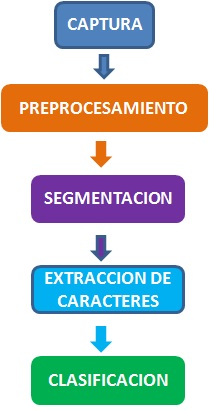
\includegraphics[width=0.3\textwidth]{EsquemaBasicoRecPatronesPrev}
  \caption{Arquitectura utilizada.}
  \label{fig1:SW}
\end{figure}
%\end{quotation}

\begin{itemize}\itemsep=0pt
\item  \textbf{Captura.-} Consiste en obtener la imagen de las cromosomas(Figura 3).
\begin{figure}
  \centering
    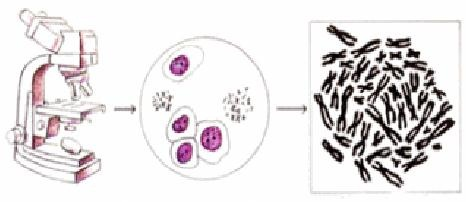
\includegraphics[width=0.5\textwidth]{1_Captura}
  \caption{Etapa de captura de los cromosomas.}
  \label{fig2:EBRP}
\end{figure}

\item  \textbf{Preprocesamiento.-} Consiste en analizar la imagen obtenida en la etapa anterior, eliminando la información irrelevante (o ruido) para el estudio.
\item  \textbf{Segmentación.-} Permite la diferenciar entre los cromosomas y el fondo dentro de la metafase celular. La segmentación consta de las etapas de binarización, la limpieza de objetos e impurezas, la separación de cromosomas unidos o traslapados y la corrección de algunos cromosomas recortados o incompletos producto de la binarización inicial.\\
La segmentación automática de imágenes de metafase tiene una larga historia, pero en sus inicios se usaban células en estado avanzado de la metafase.
En esta fase los cromosomas están contraídos y los cruces y solapamientos son raros, haciendo que la segmentación sea más sencilla. Más tarde los citogenetistas empezaron a usar imágenes de fases iniciales de la metafase o fases avanzadas de la profase, que ofrecen imágenes en las que se ven más detalles, y cromosomas con más bandas. Esto provoca que los cromosomas se vean más largos, haciendo que sea muy común que haya cruces o solapamientos. No es raro encontrar clústeres de diez o más cromosomas como se ve en la Figura 4, haciendo que sea muy importante un algoritmo para separar esos clústeres.\\

\begin{figure}
  \centering
    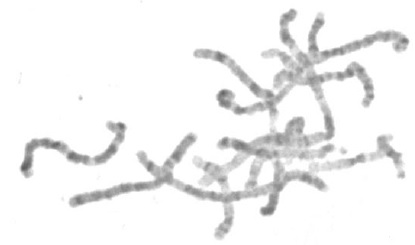
\includegraphics[width=0.5\textwidth]{4_Segmentacion}
  \caption{Ejemplo de cluster de cromosomas.}
  \label{fig4:Cluster}
\end{figure}

Se destaca la importancia de realizar un preprocesado de la imágen anterior a la segmentación, para realzar la imagen y eliminar el ruido que pueda tener para obtener una mayor calidad de detalle de los cromosomas.\\
Los métodos más simples para segmentación de cromosomas están basados en umbrales  \cite{135}, pero estos no son suficientes para separar los grupos de cromosomas concentrados.\\
La separación de cromosomas que se tocan sin cruzarse se realiza encontrando una línea de corte entre las dos, para las solapadas, en cambio, es necesario encontrar dos pares de cortes más o menos perpendiculares.\\
Se desarrollaron más técnicas para abordar este problema como las basadas en descomposiciones de forma fuzzy-logic \cite{136} o las region growing \cite{137}, aunque demostraron no ser muy eficaces.\\
En los últimos años se han hecho grandes avances en este tema, y se han presentado ideas para afrontar el problema como: concavidades de forma, pale paths (entre los cromosomas que se tocan), la esqueletización, validación
de forma...\\

\item  \textbf{Extracción de características.-} En esta fase se escogen las características a extraer de las imágenes de los cromosomas segmentados en la fase anterior, para crear la matriz de características que se usará para crear y entrenar el modelo de clasificación.\\
La primera característica que buscan los expertos a la hora de realizar el cariotipado es el tamaño. Dependiendo del tamaño son capaces de clasificar los cromosomas en pequeños grupos. \cite{131}. Después buscan características como el índice del centrómero (ratio entre el brazo corto del cromosoma y la longitud total) o la posición de las bandas características. Con este método el experto puede hacer el cariotipado de manera fiable.\\
También pueden utilizar la ayuda de un ideograma, un esquema en el que se puede ver el patrón de bandas que caracteriza a cada cromosoma, como se ve en la Figura 5. Estos ideogramas pueden tener diferentes resoluciones, mostrando más o menos bandas.

\begin{figure}
  \centering
    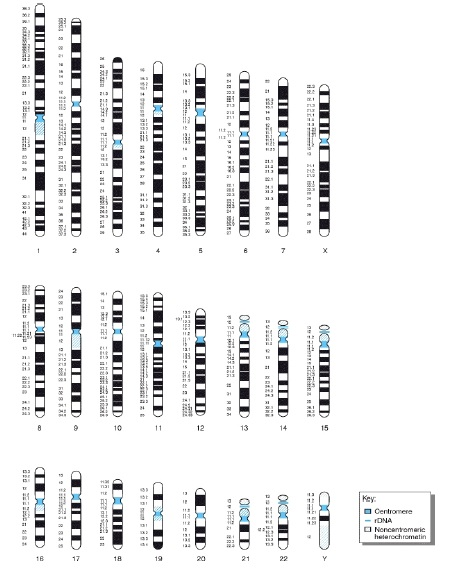
\includegraphics[width=0.3\textwidth]{5_Ideograma}
  \caption{Ejemplo de un ideograma.}
  \label{fig5:idiograma}
\end{figure}

Hoy en día existen softwares de cariotipado que usan resoluciones de 850 bandas.\\
Las características morfológicas habituales en cromosomas humanos incluyen parámetros como el área, perímetro, longitud, ratio entre el brazo corto y el largo etc. \cite{138}, pero éstos no tienen en cuenta los patrones de bandas de los cromosomas, y algunos experimentos han demostrado la eficacia de los perfiles de bandas a la hora de hacer la clasificación. \\
Generalmente se diferencian dos grupos de características:\\
\begin{itemize}\itemsep=0pt
\item  Características morfológicas.
\item  Características de textura.
\end{itemize}

Las características morfológicas aportan información de la forma y tamaño del cromosoma, pero éstas suelen ser variables, por lo que no son suficientes para realizar la clasificación completa, aunque son usadas para clasificar los cromosomas en los grupos Denver \cite{138} \\

\begin{figure}
  \centering
    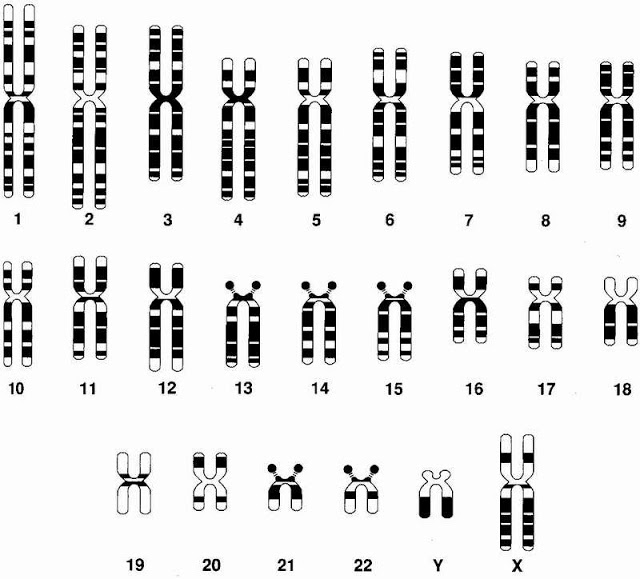
\includegraphics[width=0.4\textwidth]{6_denver}
  \caption{Representación de los grupos de Denver.}
  \label{fig6:denver}
\end{figure}



\item  \textbf{Clasificación.-} En el cariotipo humano se ha establecido en grupos de cromosomas.\\

%\end{quotation}


%\begin{quotation}
Finalmente, la implementación de estas etapas se realizará mediante algunas herramientas de desarrollo de código libre que incluyen un marco de trabajo que representa una alternativa importante con respecto al software comercial. Con estas herramientas es posible desarrollar proyectos de investigación interesantes sin que esto represente un desembolso significativo para las instituciones participantes. Una alternativa de herramientas de código libre es el OpenCV (Open Computer Vision), la cual es una biblioteca multiplataforma libre que contiene una gran cantidad de operadores de procesamiento digital de imágenes. Con respecto a esta herramienta,  Kaehler \cite{110} es una referencia bibliográfica muy importante dado que documenta ampliamente el uso de los componentes de la biblioteca. Otra de las herramientas de código libre que podría ser utilizada para la parte de clasificación requerida en el proyecto es WEKA (Waikato Environment for Knowledge Analysis), la cual es un software para aprendizaje automático y minería de datos. Una de las referencias más citadas con respecto a esta herramienta es Frank \cite{105}, la cual ha sido ampliamente consultada en diferentes artículos como una referencia importante con respecto a los algoritmos de clasificación disponibles en esta herramienta.\\
%\end{quotation}

%\begin{quotation}
Dado que el uso de este tipo herramientas computacionales es de gran utilidad para la sociedad es importante que diferentes servicios de salud tengan acceso a él.\\

Para realizar el proceso de análisis se propone el uso de un Servicio Web el cual se utilizará para que se pueda subir la imagen a analizar, poder procesarla y regresar los resultados en reporte en archivo PDF.\\
%\end{quotation}

%\begin{quotation}
Las ventajas que se tienen de realizar el proceso de esta manera son las siguientes:
%\end{quotation}

\begin{itemize}\itemsep=0pt
\item  Se puede atender a cualquier hora sin necesidad de tener a una persona dedicada a la realización del proceso de segmentación de la imagen enviada.\\
\item No es necesario que el paciente o la persona que requiera hacer el análisis se tenga que trasladar de su localidad, ya que el servicio de intenet se ha extendido 
ampliamente en el territorio nacional llegando a poblaciones rurales donde no existen centros de salud especializados.\\
\item El punto anterior nos lleva a un ahorro en gastos de transportación y alimentación que tendrían que desembolsar las personas si quisieran trasladarse a un centro de salud que lleve a cabo este proceso.\\
\item Los servicios de salud pueden hacer uso del Servicio Web para beneficio de sus derechohabientes.\\
\end{itemize}

%\begin{quotation}
Antes de continuar, vamos a definir el concepto básico de un "Servicio Web". Un servicio web es una interfaz de red que puede acceder a la funcionalidad de una aplicación, usando tecnologías de Internet (ver Apéndice B). \\ % \cite{119}\\
%\end{quotation}



%\begin{quotation}
Debido a que en este proyecto el objetivo es que cualquier persona pueda subir una imagen de un cariotipo y mediante un procesamiento e interacción con un servicio Web se pueda obtener un reporte del cariotipo analizado se va a usar un Servicio Web para Análisis (WSA).\\
%\end{quotation}

%\begin{quotation}
Para lograr lo comentado, se utilizará un esquema cliente - servidor como se muestra en la Figura 7, a realizar compresión de imágenes. Las imágenes se han convertido en un área muy importante de la informática. Hoy en día surgen más entornos gráficos orientados a múltiples aplicaciones. El uso de las imágenes se ha incrementado con el desarrollo de la informática, de igual forma su resolución (y por tanto tamaño), de ahí la necesidad de compactarlas para reducir la cantidad de datos a enviar por la web. La compresión (Paso 1, Figura 7)se basa en la eliminación de datos redundantes; dicho de otra forma, equivale a transformar una distribución bidimensional de pixeles en un conjunto de datos estadísticos sin correlacionar. Esta transformación (compresión) es aplicada a las imágenes antes de que sean almacenadas o antes de ser enviadas, por ejemplo vía red o internet. \\
%\end{quotation}

%\begin{quotation}
Con la compresión de imágenes se trata de minimizar el número de bits para representar una imagen. Las aplicaciones de la compresión de imágenes son principalmente la transmisión y almacenamiento de información. En trasmisión, sus principales aplicaciones son la televisión, el radar, redes de computadoras entre otras. En almacenamiento, la compresión de imágenes se utiliza sobre documentos, imágenes de satélite, imágenes médicas. Debido a lo comentado es que se requiere un procedimiento para realizar la compresión para su envío mediante un Servicio Web  (Paso 2, Figura 7) y sin pérdida de información relevante, y así poder llevar a cabo el cariotipo. El flujo de funcionamiento de la aplicación se muestra en la figura 7. \\

\begin{figure}
  \centering
    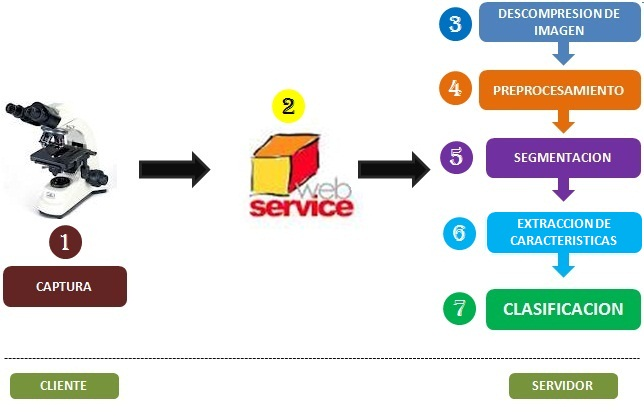
\includegraphics[width=0.9\textwidth]{7_FlujoFuncionamiento2}
  \caption{Flujo de funcionamiento de la aplicación}
  \label{fig7:FFA}
\end{figure}
%\end{quotation}

%\begin{quotation}
El Servicio Web tendrá una interacción con el proceso investigadores de la Universidad Politécnica de Victoria (UPV) en conjunto con investigadores del Hospital Infantil de Tamaulipas (HIT).\\
%\end{quotation}

%\begin{quotation}
Una vez que la imágen llega al servidor donde se encuentra instalada la aplicacion para la realización del cariotipo, se procede a descomprimir la imagen que fue comprimida durante el envío (Paso 3, Figura 7). El prepocesamiento (Paso 4, Figura 7) consiste en el alizado de la iluminación, debido a que las imágenes tienen desmedrada la iluminación y contienen ruido.\\
%\end{quotation}

%\begin{quotation}
Con la segmentación (Paso 4, Figura 7) se hace la evaluación geométrica de los cromosomas y sus intersecciones para lograr la separación de los mismos. La extracción de características (Paso 5, Figura 7) lleva a cabo la evaluación de los niveles de intensidad de los cromosomas para eliminar el ruido. Esto se genera en señales de entrenamiento.\\
%\end{quotation}

%\begin{quotation}
La forma de realizar la clasificación (Paso 6, Figura 7), se explicará más adelante dentro del Marco Teórico.\\
%\end{quotation}


%\begin{quotation}
Una vez obtenido el cariotipo (ver Figura 8), se procederá a generar un reporte de apoyo a la toma de decisiones del médico solicitante del estudio.\\
%\end{quotation}

\begin{figure}
  \centering
    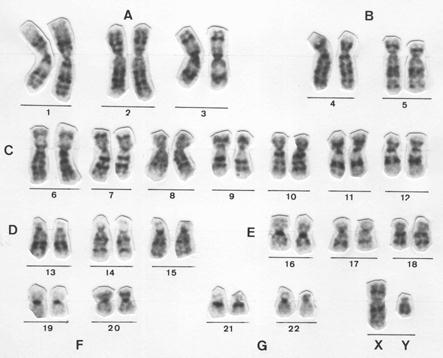
\includegraphics[width=0.6\textwidth]{8_CariotipoHumano1}
  \caption{Cariotipo Humano}
  \label{fig8:CariotipoHumano}
\end{figure}


%\begin{quotation}
Para elaborar el cariotipado es importante la clasificación de los cromosomas segmentados. El proceso a realizado en esta tesis utiliza las redes neuronales, las cuales se describen a continuación:\\
%\end{quotation}

%\begin{quotation}
Debido a que el cariotipo es una forma de análisis cromosómico que se basa en el ordenamiento estándar de los cromosomas contenidos en una célula, de acuerdo con su tamaño, localización del centrómetro \footnote{Región del cromosoma que separa los dos brazos y en la que se unen las dos cromátides. Es la región de unión a las fibras del huso acromático durante la división celular.} y patrón de bandeo \footnote{Por patrón de Bandeo se entiende el conjunto de bandas transversales de tamaño en intensidad de tinción diferentes que aparecen sobre cromosomas determinados según el modelo de distribución que depende del tinte utilizado}, éste será realizado por los investigadores de la UPV.\\

Posteriormente se realizará el proceso de clasificación. Existen diferentes tipos de técnicas para la clasificación de cromosomas por ejemplo Benoit Legrand et al. \cite{132}, proponen la técnica basada en tiempo de deformación dinámico para determinar la longitud y el perfil de densidad que son características comunes que se utilizan en la clasificación de los cromosomas.\\

Gunter Ritter \cite{133} se basa en una combinación de dos fases, una fase puramente basado en reglas y una fase impulsada por análisis discriminante restringida, pero con la desventaja que no puede realizar la clasificación de los cromosomas con información parcial, que sucede cuando los cromosomas se ocluyen entre si, por otro lado se propone el uso de redes neuronales artificiales:\\
%\end{quotation}

%\begin{quotation}
Las redes neuronales tambien denominadas redes neuronales artificiales (RNA)son sistemas ideados como abstracciones de las estructuras neurobiológicas (cerebros) encontradas en la naturaleza y tienen la característica de ser sistemas desordenados capaces de guardar información.
 \footnote{info.fisica.uson.mx/arnulfo.castellanos/archivos/html/quesonredneu.htm}\\
%\end{quotation}

%\begin{quotation}
No existe un definición general de una red neuronal artificial, existiendo diverentes según el texto ó artículo consultado; de las que podemos mencionar:
%\end{quotation}

\begin{itemize}\itemsep=0pt
\item Una red neuronal es un modelo computacional, paralelo, compuesto de unidades procesadoras adaptativas con una alta interconexión entre ellas.  \cite{126}\\
\item Modelos matemáticos desarrollados para emular el cerebro humano. \cite{127}\\
\item Sistema de procesamiento de información que tiene características de funcionamiento comunes con las redes neuronales biológicas. \cite{128}\\
\end{itemize}


%\begin{quotation}
Las RNA al margen de parecerse al cerebro presentan una serie de características
propias del cerebro. Por ejemplo las RNA aprenden de la experiencia, generalizan de
ejemplos previos a ejemplos nuevos y abstraen las características principales de una
serie de datos. \cite{124}
%\end{quotation}

\begin{itemize}\itemsep=0pt
\item  \textbf{Aprender.-} Adquirir el conocimiento de una cosa por medio del estudio, ejercicio
o experiencia. Las RNA pueden cambiar su comportamiento en función del entorno. Se
les muestra un conjunto de entradas y ellas mismas se ajustan para producir unas salidas
consistentes.
\item  \textbf{Generalizar.-} Extender o ampliar una cosa. Las RNA generalizan
automáticamente debido a su propia estructura y naturaleza. Estas redes pueden ofrecer,
dentro de un margen, respuestas correctas a entradas que presentan pequeñas
variaciones debido a los efectos de ruido o distorsión.
\item  \textbf{Abstraer.-} Aislar mentalmente o considerar por separado las cualidades de un
objeto. Algunas RNA son capaces de abstraer la esencia de un conjunto de entradas que
aparentemente no presentan aspectos comunes o relativos.
\end{itemize}

%%\begin{quotation}
%El modelo de funcionamiento de una neurona real se presenta en la Figura 5. \\
%%\end{quotation}
%
%%\begin{quotation}
%Matemáticamente su representación  se  puede ver en la Figura 6. \\
%%\end{quotation}
%
%
%\begin{figure}
%  \centering
%    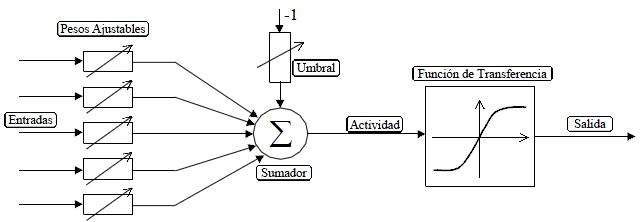
\includegraphics[width=0.9\textwidth]{ModeloNeurona}
%  \caption{Modelo de funcionamiento de una neurona real}
%  \label{fig5:MN}
%\end{figure}
%
%
%\begin{figure}
%  \centering
%    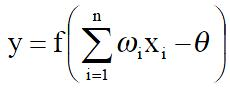
\includegraphics[width=0.3\textwidth]{ModeloNeuronaFormula}
%  \caption{Modelo de Neurona Entrada/Salida}
%  \label{fig6:MN}
%\end{figure}

%\begin{quotation}
La estructura de la red neuronal le permite la resolución de problemas que necesitarían gran cantidad de tiempo en computadoras comunes. Aparte de este hecho aparecen propiedades que las hacen atractivas para ser usadas en una gran cantidad de problemas prácticos \cite{125}
%\end{quotation}

\begin{itemize}\itemsep=0pt
\item  \textbf{Son sistemas distribuidos no lineales.-} Una neurona es un elemento no lineal por lo que una interconexión	 de ellas (red neuronal) también será un dispositivo no lineal. Esta propiedad permitirá la simulación de sistemas no  lineales y caóticos, simulación que, con los sistemas clásicos lineales, no se puede realizar.
\item  \textbf{Son sistemas tolerantes a fallas.-} Una red neuronal, al ser un sistema distribuido, permite el fallo de algunos elementos individuales (neuronas) si alterar significativamente la respuesta total del sistema.
\item  \textbf{Adaptabilidad.-} Una red neuronal tiene la capacidad de modificar los parámetros de los que depende su funcionamiento de acuerdo con los cambios que se produzcan en su entorno de trabajo (cambios en las entradas, presencia de ruido, etc).
\item  \textbf{Establecen relaciones no lineales entre datos.-} Las redes neuronales son capaces de relacionar dos conjuntos de datos. Comparando con los métodos estadísticos clásicos que realizan la misma misión tienen como principal ventaja que los datos no tienen por que cumplir las condiciones de linealidad, gausianidad y estacionariedad. \cite{129}
\item  \textbf{Posibilidad de implementación en integración en escala muy grande.-} Esta posibilidad permite que estos sistemas puedan ser aplicados en sistemas de tempo real, simulando sistemas biológicos mediante elementos de silicio. \cite{130}
\end{itemize}

%\begin{quotation}
Hasta aqui se ha presentado la parte principal de esta tesis, se ha visto la forma en que se va a interactuar con los investigadores de la Universidad Politécnica de Victoria (UPV) y los investigadores del Hospital Infantil de Tamaulipas (HIT).\\

Como se mencionó anteriormente el servicio web (Web Service) que se va a implementar cumple la función de realizar la compresión/descompresión de la imagen de los cromosomas para poder transferirlo al proceso realizado por los investigadores de la UPV y posteriormente generar el estidio del cariotipo.
%\end{quotation}




%%%%%%%%%%%%%%%%%%%%%%% METODOLOGIA
\newpage
\chapter{Metodología}\label{capIII}

En esta sección se describe la arquitectura diseñada para la solución del problema, además, 

\section{Propuesta de solución}\label{metodo}

La metodología de investigación que se llevó a cabo durante el desarrollo de la presente tesis se dividió en 2 etapas:

\begin{itemize}
\item Durante la primera se investigó acerca de los tipos de servicios web, las estrategias y el software requerido existentes para llevar a cabo implementación. En este punto se revisaron las arquitecturas existentes para SOAP y REST.\\

SOAP (siglas de Simple Object Access Protocol, Figura 9) es un protocolo estándar que define cómo dos objetos en diferentes procesos pueden comunicarse por medio de intercambio de datos XML. SOAP fue creado por Microsoft, IBM y otros y está actualmente bajo el auspicio de la W3C.\\


Los objetivos primordiales de SOAP, son:\\

a) Establecer un protocolo estándar de invocación de servicios remotos, basado en protocolos estándares de Internet: HTTP (Hiper Text Transport Protocol) para la transmisión y XML (eXtensible Markup Language) para la codificación de datos.\\

b) Independencia de plataforma, lenguaje de desarrollo e implementación (modelo de objetos).\\

El protocolo de comunicación HTTP es el empleado intrínsecamente para la conexión sobre Internet. Garantiza que cualquier cliente con un navegador estándar pueda conectarse con un servidor remoto. La transmisión de datos se empaqueta (serializa) con XML.\\

\begin{figure}
  \centering
    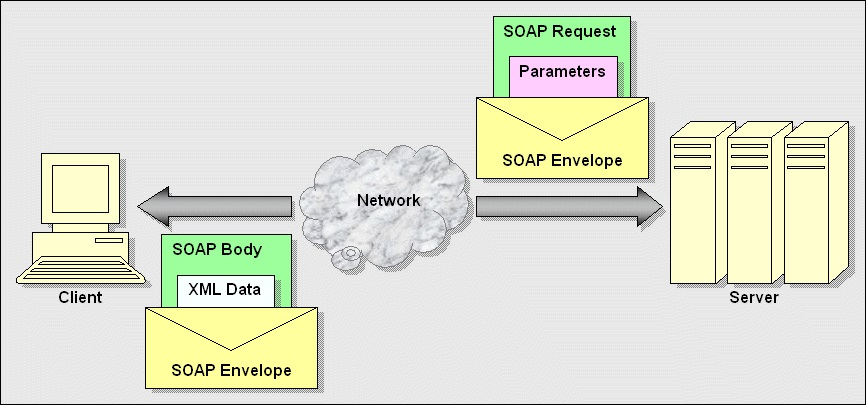
\includegraphics[width=0.9\textwidth]{9_soap}
  \caption{Flujo de SOAP}
  \label{fig9:soap}
\end{figure}

La especificación SOAP menciona que las aplicaciones deben ser independientes del lenguaje de desarrollo, por lo que las aplicaciones cliente y servidor pueden estar escritas con HTML, DHTML, Java, Visual Basic u otras herramientas y lenguajes disponibles.\\


REST define un set de principios arquitectónicos por los cuales se diseñan Servicios Web haciendo foco en los recursos del sistema, incluyendo cómo se accede al estado de dichos recursos y cómo se transfieren por HTTP hacia clientes escritos en diversos lenguajes. REST emergió en los últimos años como el modelo predominante para el diseño de servicios. (Figura 10)\\

\begin{figure}
  \centering
    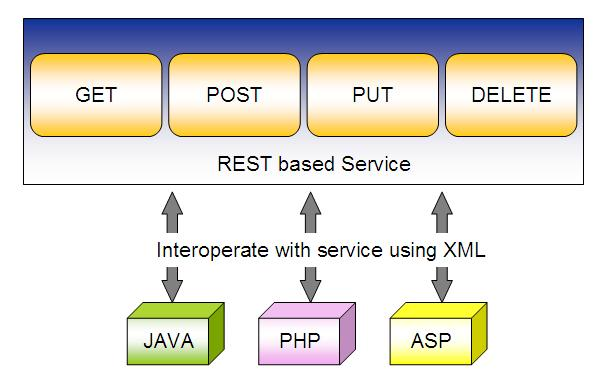
\includegraphics[width=0.9\textwidth]{10_rest}
  \caption{REST}
  \label{fig10:rest}
\end{figure}
Una implementación concreta de un servicio web REST sigue cuatro principios de diseño fundamentales:\\

a)Utiliza los métodos HTTP de manera explícita\\
b)No mantiene estado \\
c)Expone URLs con forma de directorios \\
d)Transfiere XML, JavaScript Object Notation (JSON)\\

Una de las caraterísticas claves de los servicios web REST es el uso explícito de los métodos HTTP, siguiendo el protocolo definido por RFC 2616. Por ejemplo, HTTP GET se define como un método productor de datos, cuyo uso está pensado para que las aplicaciones cliente obtengan recursos, busquen datos de un servidor web, o ejecuten una consulta esperando que el servidor web la realice y devuelva un conjunto de recursos.\\

REST hace que los desarrolladores usen los métodos HTTP explícitamente de manera que resulte consistente con la definición del protocolo. Este principio de diseño básico establece una asociación uno-a-uno entre las operaciones de crear, leer, actualizar y borrar y los métodos HTTP.\\

Los servicios web REST necesitan escalar para poder satisfacer una demanda en constante crecimiento. Se usan clusters de servidores con balanceadores de carga y alta disponibilidad, proxies, y gateways de manera de conformar una topología serviciable, que permita transferir peticiones de un equipo a otro para disminuir el tiempo total de respuesta de una invocación al servicio web. El uso de servidores intermedios para mejorar la escalabilidad hace necesario que los clientes de servicios web REST envien peticiones completas e independientes; es decir, se deben enviar peticiones que inlcuyan todos los datos necesarios para cumplir el pedido, de manera que los componentes en los servidores intermedios puedan redireccionar y gestionar la carga sin mantener el estado localmente entre las peticiones.\\

Una petición completa e independiente hace que el servidor no tenga que recuperar ninguna información de contexto o estado al procesar la petición. Una aplicación o cliente de servicio web REST debe incluir dentro del encabezado y del cuerpo HTTP de la petición todos los parámetros, contexto y datos que necesita el servidor para generar la respuesta. De esta manera, el no mantener estado mejora el rendimiento de los servicios web y simplifica el diseño e implementación de los componentes del servidor, ya que la ausencia de estado en el servidor elimina la necesidad de sincronizar los datos de la sesión con una aplicación externa.\\

\item En la segunda etapa del proyecto se investigó sobre los métodos de compresión de imágenes, analizando los diversos métodos  existentes en la actualidad.\\

El objetivo de la compresión de imagen es reducir los datos redundantes e irrelevantes de la imagen con la menor perdida posible para permitir su almacenamiento o transmisión de forma eficiente.\\

En todos los casos siguientes el simple hecho de comprimir, produce una pérdida de calidad. En la mayoría de los casos, ésta es imperceptible al ojo humano. A la hora de almacenar una imagen, hay que guardar, además de la silueta que da forma a la imagen, los colores asociados a cada pixel.\\

Existen muchas formas de hacerlo, dando lugar a los distintos formatos de imagen. Algunos, como el formato BMP, son muy utilizados. Este formato, sin embargo, ocupa demasiado espacio (un dibujo con 256 colores puede extenderse hasta los 900 Kb).\\
El ojo humano responde con diferente sensibilidad a la información visual que recibe. La información a la que es menos sensible se puede descartar sin afectar la percepción de la imagen, suprimiendo así lo que se denomina redundancia visual.
Fue así como surgieron algunos formatos de imagen que utilizan distintas técnicas de compresión.\\

Aunque su número es muy elevado, los más prácticos son, sin duda, los formatos PCX, GIF y JPEG. Todos ellos pueden convertir cualquier imagen, por compleja que sea, en un archivo de imagen que no suele superar los 100 Kb, a costa de perder un mínimo de calidad (métodos lossy) que, en la mayoría de los casos, no puede ser apreciada por el ojo humano. Para comprimir una imagen generada digitalmente, se utilizan las técnicas descritas a continuación.\\

\textbf{ a)Transformada discreta del coseno.}- En este tipo de transformación, la imagen de entrada se divide en bloques de NxN píxeles. El tamaño del bloque se escoge considerando los requisitos de compresión y la calidad de la imagen.\\
En general, a medida que el tamaño del bloque es mayor, la relación de compresión también resulta mayor. Esto se debe a que se utilizan más píxeles para eliminar las redundancias. Pero al aumentar demasiado el tamaño del bloque la suposición que las características de la imagen se conservan constantes no se cumple, y ocurren algunas degradaciones de la imagen, como la falta de definición de los bordes. El tamaño típico de bloque es de 8x8 píxeles.\\

\textbf{ b) JPEG (Joint Photographic Experts Group).}- Fue desarrollado por expertos fotográficos trabajando juntos bajo los auspicios de ITU, ISO e IEC. JPEG está definido en el estándar internacional 10918.\\
Es el método por pérdidas más utilizado actualmente para la compresión de imágenes. Este método utiliza la transformada discreta del coseno (DCT), que se calcula empleando números enteros, por lo que se aprovecha de algoritmos de computación veloces. El JPEG consigue una compresión ajustable a la calidad de la imagen que se quiera reconstruir. Es utilizado en todos los archivos con extensión JPG. La pérdida de calidad a la hora de comprimir imágenes hace que el formato JPEG tenga una serie de limitaciones. JPEG está especialmente indicado para comprimir imágenes en color o en escala de grises, más no en blanco y negro. Igualmente, funciona mejor cuando la imagen presenta una coloración continuada y suave; las imágenes que presentan cambios bruscos de color no se comprimen demasiado bien. El proceso de compresión se basa en la definición de una gran cantidad de parámetros que determinan la calidad de la compresión, teniendo en cuenta que a mayor compresión, menor calidad, y viceversa. JPEG utiliza un algoritmo base más extensiones opcionales basadas en sistemas de compresión progresivos. El algoritmo base consta de los siguientes pasos:


\begin{itemize}\itemsep=0pt
\item  Se divide la imagen separando los componentes cromáticos de los componentes lumínicos. La razón de esto es que se pueden comprimir más los componentes cromáticos sin que el ojo humano sea capaz de percibirlo.\\
\item Este paso sólo se realiza con las imágenes en color. El componente lumínico se deja en la resolución máxima, mientras que el componente cromático se reduce a la mitad horizontal y verticalmente (2:1). En el último caso, también puede dejarse como está (1:1), dependiendo de la calidad de compresión que se elija. Este paso reduce inmediatamente el tamaño de la imagen en 1/2 o un 1/3, sin que el ojo humano perciba esta reducción cromática..\\
\item Para cada componente, se agrupan los píxeles en grupos de 8x8. A cada bloque se le aplica una transformación Fourier, que realiza varios cambios para obtener valores medios de cromatismo y luminosidad de cada bloque. Los coeficientes de la transformada son cuantificados con base en un nivel de umbral para obtener el mayor número de ceros posibles.\\
\item Cada uno de los bloques se divide en sus componentes de frecuencia, mediante lo que se llama “componente de cuantización”, y se redondea el resultado a un valor entero. Aquí es donde se produce la compresión y la pérdida de información, almacenando sólo ciertos valores de las frecuencias, mediante unas tablas de cuantización. Luego se reordena en zig-zag la matriz de coeficientes cuantificados.\\
\item Se codifica los componentes reducidos utilizando el método Huffman, el cual se encarga de transmitir los coeficientes ordenados. Para realizar la compresión, el compresor Huffman crea códigos más cortos para símbolos que se repiten frecuentemente y códigos más largos para símbolos que ocurren con menor frecuencia.\\
\item Se crea una cabecera con todos los datos técnicos de la compresión, y se almacena la imagen final en el archivo. Con estos datos, el descompresor -es decir, el programa de edición que muestra la imagen- puede realizar el proceso contrario.\\
\end{itemize}
Los algoritmos progresivos permiten aumentar la calidad, utilizando tablas variables de cuantización que mantienen la calidad en las zonas más visibles y la reduce en las menos visibles, así como distintos sistemas de refinamiento para mejorar la calidad de la imagen.\\

\end{itemize}

%%%%%%%%%%%%PACO FALTA PORNER LOS RESULTADOS!!!!%%%%%%%%%%%%


%%%%%%%%%%%%%%%%%
%%%%%%%%%%%%%%%%% CONCLUSIONES
\chapter{Conclusiones}\label{conclusiones}
Como profesional del área del sistemas consideró importante aplicar los conocimientos a proyectos que nos ayuden a mejor nuestra calidad de vida así como desarrollar aplicaciones que ayuden a gente de otras áreas a optimizar su procesos.\\

Es por eso que el propósito de la presente tesis fue poder generar una aplicación que sirva de apoyo a los médicos rurales en la detección de problemas de índole genético durante la etapa de la concepción.\\

El tema fue realizado y escogido para un área social donde la población tiene muchas limitantes en su calidad de vida y muchas veces el poder relizarse un cariotipo resulta difícil para ellos, ya que implica tener que trasladarse de su comunidad a una ciudad más grande que cuente con el equipo y personal capacitado para el estudio requerido \\

Para poder desarrollar la aplicación, como se comentó se tuvieron que llevar a cabo pruebas con las diversas tecnologías que había y que estan en desarrollo para los servicios web. Los cuales por ser parte de un área como es de sistemas y computación, está en constante evolución y las actualizaciones a las mismas cambian rápidamente, asi mismo para la compresión de imágenes, ya que todos los días en un mundo globalizado donde esta área es parte primirdial se busca nuevas arquitecturas, tecnologías y herramientas que ayuden a optimir los recursos con los que contamos y que reduzcan costos en los procesos llevados a cabo con herramientas tecnológicas.\\

En las pruebas relizadas para poder realizar este estudio con el software desarrollado, resultaron muy sencillas debido a que no se requieren conocimientos mayores de computación, con el hecho de que la persona sepa utilizar un browser para internet es suficiente para poder llevar a cabo el cariotipo.\\

%%%%%%%%%%%%%%%%%
%%%%%%%%%%%%%%%%%%%%%%% CRONOGRAMA
\section{Cronograma de actividades}\label{cronograma}
%\begin{quotation}
%Cronograma de Actividades
%\end{quotation}
Las actividades que se realizaron en cada etapa de esta tesis se muestran a continuación:\\


\begin{center}
%\begin{sideways}
\scalebox{0.70}{
\begin{tabular}{|l|c|c|c|c|c|c|}
\hline
\textbf{\centering Actividad} & \textbf{Bim-I} & \textbf{Bim-II} & \textbf{Bim-III} & \textbf{Bim-IV} & \textbf{Bim-V} & \textbf{Bim-VI} \\
\hline
Investigar Estado del Arte (Cariotipado) & \cellcolor{black} & \cellcolor{black} &   &   &   &  \\ 
\hline
Investigación sobre Servicios Web &  & \cellcolor{black} &  \cellcolor{black}  &   &   &  \\
\hline
Inv. Métodos de Compresión de Imágenes & \cellcolor{black} &  \cellcolor{black} &  &  &  &  \\
\hline
Implementación del WebService &   &  & \cellcolor{black} &    &    &  \\
\hline
Implementación del Métodos de Compresión &   &   & \cellcolor{black} &   &   &  \\
\hline
Diseño e implementación de interfaz &   &   &  & \cellcolor{black} & \cellcolor{black} &  \\
\hline
Pruebas &   &   &  \cellcolor{black}  & \cellcolor{black} &  & \\
\hline
Artículo &   &   &   &  \cellcolor{black}  & \cellcolor{black}  &  \\
\hline
Reporte de Beca &   & \cellcolor{black}  & \cellcolor{black}  &  \cellcolor{black}   & \cellcolor{black} & \cellcolor{black} \\
\hline
Tesis &   & \cellcolor{black} &   & \cellcolor{black}  &   &   \cellcolor{black} \\
\hline
Defensa del examen &   &   &   &  &   &  \cellcolor{black}\\
\hline
\end{tabular}}
%\end{sideways}
\end{center}


\newpage

%%%%%%%%%%%%%%%%%%%%%%% APENDICE A

\section{Apendice A}\label{apendicea}
\begin{itemize}\itemsep=0pt
\item  \textbf{Cromosomas Grupo A.-} A este grupo aparecen los cromosomas más grandes del cariotipo humano: Pertenece a él los pares de cromosomas 1, 2 y 3.\\

\begin{itemize}\itemsep=0pt
\item  {Cromosoma 1.-} es el más grande de todos y metacéntrico. 
\item  {Cromosoma 2.-} es submetacéntrico. 
\item  {Cromosoma 3.-} es metacéntrico. 
\end{itemize}

\item  \textbf{Cromosomas Grupo B.-} En este grupo se incluyen los pares de cromosomas 4 y 5. son cromosomas muy submetacéntricos y de tamaño muy similar. Alteraciones con estos cromosomas se ha demostrado que provocan grandes síndromes citogenéticas.
\item  \textbf{Cromosomas Grupo C.-} A este grupo pertenecen los cromosomas 6, 7, 8, 9, 10, 11, 12 y el gonosoma X. Este es el grupo más complejo que todos la mayoria de los cromosomas son bastante submetacéntricos.\\
\begin{itemize}\itemsep=0pt
\item  {Cromosoma 6.-} es submetacéntrico. 
\item  {Cromosoma 7.-} es menos submetacéntrico. 
\item  {Cromosoma 8.-} es muy submetacéntrico. 
\item  {Cromosoma 9.-} es menos submetacéntrico. 
\item  {Cromosoma 10.-} es muy submetacéntrico. 
\item  {Cromosoma 11.-} es menos metacéntrico. 
\item  {Cromosoma 12.-} es muy submetacéntrico. 
\item  {Cromosoma X.-} es submetacéntrico y tiene un tamaño medio entre el cromosoma 6 y el 7. 
\end{itemize}

\item  \textbf{Cromosomas Grupo D.-} Este grupo está compuesto por los cromosomas 13, 14 y 15. Son cromosomas acrocéntricos. Además, presentan constricciones secundarias, que dan lugar a pequeños satélites poco visibles a microscopía electrónica donde se encuentran los genes nucleolares.
\item  \textbf{Cromosomas Grupo E.-} En este grupo incluimos 16, 17 y 18. Los presentan un tamaño similar:\\
\begin{itemize}\itemsep=0pt
\item  {Cromosoma 16.-} es metacéntrico. 
\item  {Cromosoma 17.-} es submetacéntrico. 
\item  {Cromosoma 18.-} es muy submetacéntrico. 
\end{itemize}

\item  \textbf{Cromosomas Grupo F.-} Este grupo esta formado por los cromosomas 19 y 20. Entre ellos no se diferencían prácticamente. Por su tamaño y por el hecho de que son metacéntricos se les denomina "pequeñas cruces".
\item  \textbf{Cromosomas Grupo G.-} Los cromosomas 21 y 22, así como gonosoma Y forman este grupo de cromosomas. Son los cromosomas más pequeños del cariotipo.
\begin{itemize}\itemsep=0pt
\item  {Cromosomas 21 y 22.-} son acrocéntricos y tienen satélites con genes nucleolares. 
\begin{itemize}\itemsep=0pt
\item  El cromosoma 21 es realmente el cromosoma más paqueño del cariotipo, pero está colocado de esta manera por acuerdo internacional, ya que históricamente se colocó en esa posición, es el responsable del síndrome de Down, ayudó al despegue de la citogenética. 
\end{itemize}

\item  {Cromosoma Y.-} es submetacéntrico y presenta un tamaño variable. Sus dos cromátidas se sitúan muy paralelas y no divergentes. Además, esta formado por heterocromatina constitutiva porque no tiene genes. 
\end{itemize}

\end{itemize}


\end{itemize}
%%%%%%%%%%%%%% APENDICE B
\newpage
\section{Apendice B}\label{apendiceb}


%%%%%%%%%%% inicio enero2013

Los \textbf{Servicios Web} (Web Services en inglés ) son un estandar de comunicación entre procesos y componentes, diseñado para ser multiplataforma y multilenguaje, es decir, no importa en que lenguaje esté programado un Servicio Web o en qué plataforma esté corriendo, ya sea Windows, Unix o Linux éstos serán accesibles y utilizables para aplicaciones desarrolladas en otras plataformas o lenguajes de programación. Anteriormente se utilizaban otros estándares como DCOM (Distributed Common Object Model) introducido por Microsoft e implementado por otras plataformas, y CORBA (Common Object Request Broker Architecture) introducido por el OMG (Object Management Gruop) e implementado por diferentes plataformas. Estos estándares tenían bastantes problemas de configuración, especialmente en entornos en que se encontraban firewalls de por medio en los cuales era imposible (debido a estándares de seguridad de muchas compañías) habilitar ciertos puertos de comunicación para que estos funcionaran. De esta manera la preferencia para utilizar el puerto 80 de HTTP (Hypertext Tranfer Protocol, Protocolo de Tranferencia de Hipertexto) que normalmente se encuantra habilitado en la mayoria de los servidores y firewalls debido al uso de navegadores y servideores web, no traería complicaciones el uso de una tecnología que utilice este protocolo y puerto TCP/IP.\\

El desarrollo y la programación de sistemas prientados a objetos o componentes nos ha llevado a lo largo del tiempo a tener la necesidad de reutilizarlos en diferentes proyectos. Hasta la existencia de los Servicios Web la reutilización nos limitaba a un lenguje de programación o a una plataforma en particular, por lo que los Servicios Web nos facilitan la reutilización de funciones de una aplicación en distintas plataformas o lenguajes ya sea para un uso personal en distintos proyectos, para comercializarlos o adquirir prestaciones de terceros. \cite{134}\\

Para conocer cómo se realiza el intercambio de mensajes en los Web Services debemos primero saber cuales son los elementos fundamentales que lo componen. Estos son el XML, SOAP, WSDL, y UDDI.\\

\subsection{XML}\label{xml}
XML (Extendible Markup Languaje, Lenguaje Extendido de Marcas) es un lenguaje utilizado para definir formatos de documentos o mensajes. Estos están compuestos por Tags (palabras entre caracteres \textbf{<} y \textbf{>}). Estos tipos de documentos han sido aceptados y adoptados por la mayoria de fabricantes de software para proveer extensibilidad de los datos debido a que no está atado a ninguna plataforma o lenguaje de programación. Podemos ver que XML es muy similar al HTML (Hypertext Markup Languaje, Lenguaje de Marcado de Hipertexto), pero sin embargo el XML es más estricto ya que por cada tag abierto deberemos tener un tag que lo cierre, debido a que si no se cierra éste no podrá ser interpretado por los parsers (clases utilizadas para el manejo de documentos XML)\\

Ha ganado muchísima popularidad en los ultimos a  nos debido a ser un estándar abierto y libre, creado por el Consorcio World Wide Web, W3C (los creadores de la www), en colaboración con un panel que incluye representantes de las principales compañias productoras de software.\\

Aparte de los tags hay otras restricciones y validaciones que los documentos XML deberán cumplir, eso depende de un archivo de definiciones llamado DTD (Document Type Definitions, Definicón del tipo de Documento) o de un archivo de esquemas de XML. En estos archivos DTDs podremos definirsi un elemento (también llamado nodo) deberá al menos aparecer una vez, una o más veces, una a ninguna vez. a su vez, cada elemento podrá tener uno o más atributos eso depende también del archivo de definiciones o esquema. Estos documentos XML son la base de los documentos WSDL y SOAP, base de los Servicios Web. (Figura 11)\\

\begin{figure}
  \centering
    \includegraphics[width=0.4\textwidth]{11_xml}
  \caption{XML}
  \label{fig11:xml}
\end{figure}

%\begin{figure}
%  \centering
%    \includegraphics[width=0.9\textwidth]{11_xml}
%  \caption{REST}
%  \label{fig10:rest}
%\end{figure}

\subsection{WSDL}\label{wsdl}
WSDL (Web Services Description Languaje, Lenguaje de Descripción de Servicios Web) es un documento XML que se utiliza para describir mensajes SOAP y cómo estos mensajes son intercambiados. Es decir, supongamos que creamos un Servicio Web y queremos que otras apliaciones lo utilicen, las otras aplicaciones deberán acceder a un documento WSDL en donde podrán conocer los métodos que expone nuestro Servicio Web y cómo acceder a ellos, es decir, cuales son los nombres de los métodos y qué tipos de parámetros espera para cada uno de ellos. Todo documento WSDL está compuesto por un elemento raíz llamado \textbf{definitions} que a su vez esta compuesto por los siguientes elementos:\\

\begin{itemize}\itemsep=0pt
\item \textbf{types} define el tipo de esquema a ser utilizao, usualmente XML.
\item \textbf{message} en este elemento se definen los mensajes de entrada y salida en forma abstracta entre el servidor y el cliente. Normalmente habrá varios elementos de este tipo por cada protocolo (HTTP, SOAP) y para cada Web Method.
\item \textbf{portType} define los tipos de mensajes a intercambiar entre el cliente y el servidor. Este puede ser de los tipos \textbf{Request-response}, en el cual por cada requerimiento se envía una respuesta, o \textbf{One-Way}, donde el Web service sólo recibe requerimentos pero no envía  respuestas; \textbf{Solicit-Response}, la inversa del Request-Response ya que el que solicita el requerimiento es el servidor en vez del cliente y por último Notification \textbf{inverso al One-Way}, donde el que manda el mensaje es sólo el servidor. (Figura 12)
\end{itemize}

\begin{figure}
  \centering
    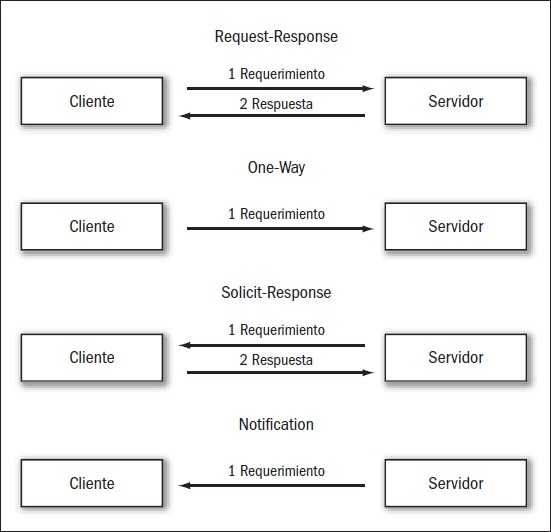
\includegraphics[width=0.4\textwidth]{12_porttype}
  \caption{Diversos portType}
  \label{figx:porttype}
\end{figure}

\begin{itemize}\itemsep=0pt
\item \textbf{binding} en este elemento se establecen las definiciones de los vínculos de los protocolos como SOAP a un tipo de vículo en particular. Por ejemplo, para el protocolo SOAP tendremos el atributo soapAction del elemento soap:operation la URL que tendremos que utilizar para invocar un Web Method.
\item \textbf{service} en este elemento se informa el punto de acceso a los servicios para cada uno de los protocolos a través de un elemento address.
\end{itemize}

\begin{figure}
  \centering
    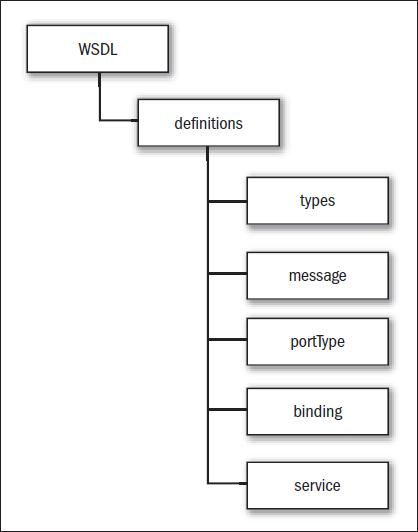
\includegraphics[width=0.4\textwidth]{13_wsdl}
  \caption{Elementos de un documento WSDL}
  \label{fig13:wsdl}
\end{figure}

Los documentos WSDL son necesarios para que cualquier lenguaje de programación pueda generar una clase llamada proxy que utilizaremos desde nuestra aplicación cliente sin necesidad de entender o parsear este tipo de documentos. (Figura 13)

\subsection{SOAP}\label{soap}
SOAP (simple Object Access Protocol, Protocolo de Acceso de Objeto Simple) es el protocolo base de los Servicios Web. Este protocolo está basado en XML y no se encuentra atado a ninguna plataforma o lenguaje de programación. A su vez, también es el protocolo más aceptado por la mayoría de las plataformas. (Figura 14)\\

\begin{figure}
  \centering
    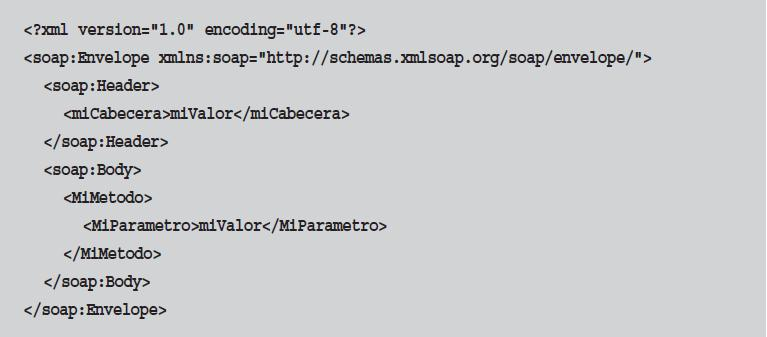
\includegraphics[width=0.6\textwidth]{14_soap}
  \caption{Código SOAP}
  \label{fig14:soap}
\end{figure}

Si bien SOAP es un protocolo, éste no es exactamente un protocolo de comunicación entre mensajes como lo es el HTTP. Básicamente, SOAP son documentos XML y necesitaremos utilizar algún protocolo para la transmisión de estos documentos como ser el protocolo HTTP o cualquier otro protocolo de comunicación capaz de transmitir texto. Los mensajes SOAP están compuestos por un tag principal llamado \textbf{envelope}, que está dicidido en una cabecera \textbf{header} y en un cuerpo o \textbf{Body}. (Figura 15)\\

\begin{figure}
  \centering
    \includegraphics[width=0.6\textwidth]{15_soapelements}
  \caption{Elementos SOAP}
  \label{fig15:elemsoap}
\end{figure}


Dentro del elemento \textbf{Body} estarán los elementos correspondientes al \textbf{Web Method} que queramos invocar y además podrá haber o no un elemento en común llamado \textbf{Fault} que nos indicará que ha ocurrido un error y la razón de éste.\\


%%%%%%%%%%% FIN enero2013

Los Servicios Web (WS, ver figura 16) pueden clasificarse de varias formas. Según la funcionalidad de los Servicios Web (Canta et al. \cite{121}) dividen a los Servicios Web en dos categorías: Servicios Web Programáticos (Programmatic Web Services, PWS) y Servicios Web Interactivos (Interactive Web Services, IWS); los primeros encapsulan la funcionalidad en la capa de negocios de las aplicaciones, mientras que los segundos la encapsulan en la interfaz de usuario o la capa de presentación. Los PWS extienden la capa lógica de negocios de una aplicación. En los Servicios Web la característica de mantenibilidad se ve reflejada a través de la simpleza de las operaciones que permiten la facilidad de cambio, análisis y pruebas; además propicia funcionalidad gracias a la posibilidad que posee el suscriptor de adecuar dichas funciones a sus requerimientos específicos. Los IWS exponen una interfaz de usuario de aplicación. Como éstos se manejan a través de la interfaz del usuario, la característica de usabilidad se ve reflejada en ellos, de acuerdo a las necesidades del negocio. Microsoft \cite{122} clasifica a los Servicios Web según la funcionalidad que el negocio desee darle al mismo:\\


\begin{figure}
  \centering
    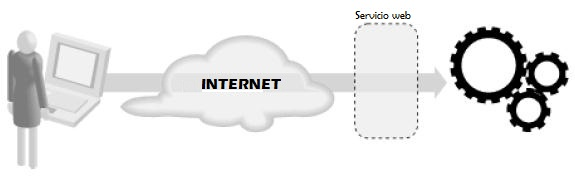
\includegraphics[width=0.7\textwidth]{16_ServicioWeb}
  \caption{Servicio Web}
  \label{fig16:SW}
\end{figure}

\begin{itemize}\itemsep=0pt
\item \textbf{Los Servicios Web Orientados a datos (Web Services Data Centric, WSDC)} que son útiles en situaciones donde deben actualizarse datos que son alterados frecuentemente. Se puede deducir que los WSDC propician la característica de eficiencia al negocio; por lo que las organizaciones que requieren de la adecuada utilización del tiempo y los recursos, ven conveniente la aplicación de este tipo de Servicio Web para obtener los beneficios esperados.\\
\item \textbf{Los Servicios Web de Colaboración (Web Service Collaboration, WSC)} son aquellos que permiten la colaboración entre todos los involucrados del negocio. Estos Servicios Web suministran la característica de interoperabilidad al negocio.\\
\item \textbf{Los Servicios Web para Análisis (Web Service Analysis, WSA)} son aquellos que reciben informes de varias empresas filiales, las ejecutan, consolidan y entregan los resultados deseados. Por lo tanto, este tipo de Servicio Web impulsa la característica de usabilidad del negocio.\\
\item \textbf{Los Servicios Web de Alertas (Web Services Alert, WSAL)} manejan situaciones de alerta más eficientemente, ya que se puede enviar mensajes de aviso a un dispositivo móvil (celular, pda, etc) para que se pueda actuar de inmediato. La característica fundamental que propicia al negocio éste tipo de Servicio Web, es la eficiencia. Los requerimientos de los usuarios establecen los criterios para seleccionar el tipo de Servicio Web que se ha de aplicar. Estos requerimientos exigen características de calidad que el usuario espera del Servicios Web. La Tabla que se muestra a continuación resume la clasificación de los servicios Web (Web Service WS) planteada anteriormente junto con la(s) característica(s) de calidad asociada(s) a cada una de ellas y traducidas al estándar ISO 9126 \cite{123}.\\
\end{itemize}

\begin{center}
%\begin{sideways}
\scalebox{0.60}{
\begin{tabular}{|l|l|l|}
\hline
\textbf{\centering Tipo de WS} & \textbf{Características de calidad del negocio} & \textbf{Según ISO/EIC 9126}\\
%%\multicolumn{3}{|c|}\textbf{Tipo de WS} & \textbf{Características de calidad del negocio} &\textbf{Según ISO/EIC 9126}\\
\hline
%%\multicolumn{3}{|l|}{PWS} & {Mantebilidad, Funcionalidad} & {Mantebilidad, Funcionalidad}\\
PWS & Mantebilidad, Funcionalidad  & Mantebilidad, Funcionalidad\\
\hline
%%\multicolumn{3}{|l|}{IWS} & {Usabilidad} & {Usabilidad}\\
IWS & Usabilidad  & Usabilidad\\
\hline
%%\multicolumn{3}{|l|}{WSDC} & {Eficiencia} & {Eficiencia}\\
WSDC & Eficiencia  & Eficiencia\\
\hline
%%\multicolumn{3}{|l|}{WSC} & {Interoperabilidad} & {Interoperabilidad}\\
WSC & Interoperabilidad  & Interoperabilidad\\
\hline
%%\multicolumn{3}{|l|}{WSA} & {Usabilidad} & {Usabilidad}\\
WSA & Usabilidad  & Usabilidad\\
\hline
%%\multicolumn{3}{|l|}{WSAI} & {Eficiencia} & {Eficiencia}\\
WSAI & Eficiencia  & Eficiencia\\
\hline
%%\multicolumn{3}{|l|}{QoS} & {Rendimiento, Fiabilidad, Seguridad} & {Rendimiento, Fiabilidad, Seguridad} \\
QoS & Rendimiento, Fiabilidad, Seguridad  & Rendimiento, Fiabilidad, Seguridad\\
\hline
\end{tabular}}
%\end{sideways}
\end{center}

%\begin{quotation}
Para poder implementar un servicio Web se cuenta con las siguientes tecnologías:\\
%\end{quotation}

\begin{itemize}\itemsep=0pt
\item  \textbf{Protocolo Simple de Acceso al Objeto (SOAP).-} Es un estándar de la World Wide Web Consortium (W3C) que describe un formato de mensaje (basado en XML) y mecanismos para intercambiar información entre aplicaciones, en un ambiente distribuido y descentralizado.\\
\item  \textbf{Lenguaje de Definición del servicio Web (WSDL).-} Es un estándar de la W3C que define un lenguaje basado en XML que permite describir la interfaz, formas de acceso y ubicación de un Servicio Web.\\
\item  \textbf{Universal Descripción, Descubrimiento e Integración (UDDI).-} Estándar de la
Advancing Open Standards for the Information Society (OASIS) que provee una forma estándar de publicar, categorizar y buscar Servicios Web.\\
\end{itemize}




%%%%%%%%%%%%%%%%%%%%%%% BIBLIOGRAFIA
\newpage
\bibliographystyle{abbrv}
%\bibliographystyle{unsrt}
%\bibliographystyle{apalike}
\bibliography{bibliografia}


\end{document}

